
%%%%%%%%%%%%%%%%%% PREAMBULE %%%%%%%%%%%%%%%%%%

\documentclass[aspectratio=169,utf8]{beamer}
%\documentclass[aspectratio=169,handout]{beamer}

\usetheme{Boadilla}
%\usecolortheme{seahorse}
\usecolortheme[RGB={245,66,24}]{structure}
\useoutertheme{infolines}

% packages
\usepackage{amsfonts,amsmath,amssymb,amsthm}
\usepackage[utf8]{inputenc}
\usepackage[T1]{fontenc}
\usepackage{lmodern}

\usepackage[francais]{babel}
\usepackage{fancybox}
\usepackage{graphicx}

\usepackage{float}
\usepackage{xfrac}

%\usepackage[usenames, x11names]{xcolor}
\usepackage{tikz}
\usepackage{pgfplots}
\usepackage{datetime}



%-----  Package unités -----
\usepackage{siunitx}
\sisetup{locale = FR,detect-all,per-mode = symbol}

%\usepackage{mathptmx}
%\usepackage{fouriernc}
%\usepackage{newcent}
%\usepackage[mathcal,mathbf]{euler}

%\usepackage{palatino}
%\usepackage{newcent}
% \usepackage[mathcal,mathbf]{euler}



% \usepackage{hyperref}
% \hypersetup{colorlinks=true, linkcolor=blue, urlcolor=blue,
% pdftitle={Exo7 - Exercices de mathématiques}, pdfauthor={Exo7}}


%section
% \usepackage{sectsty}
% \allsectionsfont{\bf}
%\sectionfont{\color{Tomato3}\upshape\selectfont}
%\subsectionfont{\color{Tomato4}\upshape\selectfont}

%----- Ensembles : entiers, reels, complexes -----
\newcommand{\Nn}{\mathbb{N}} \newcommand{\N}{\mathbb{N}}
\newcommand{\Zz}{\mathbb{Z}} \newcommand{\Z}{\mathbb{Z}}
\newcommand{\Qq}{\mathbb{Q}} \newcommand{\Q}{\mathbb{Q}}
\newcommand{\Rr}{\mathbb{R}} \newcommand{\R}{\mathbb{R}}
\newcommand{\Cc}{\mathbb{C}} 
\newcommand{\Kk}{\mathbb{K}} \newcommand{\K}{\mathbb{K}}

%----- Modifications de symboles -----
\renewcommand{\epsilon}{\varepsilon}
\renewcommand{\Re}{\mathop{\text{Re}}\nolimits}
\renewcommand{\Im}{\mathop{\text{Im}}\nolimits}
%\newcommand{\llbracket}{\left[\kern-0.15em\left[}
%\newcommand{\rrbracket}{\right]\kern-0.15em\right]}

\renewcommand{\ge}{\geqslant}
\renewcommand{\geq}{\geqslant}
\renewcommand{\le}{\leqslant}
\renewcommand{\leq}{\leqslant}
\renewcommand{\epsilon}{\varepsilon}

%----- Fonctions usuelles -----
\newcommand{\ch}{\mathop{\text{ch}}\nolimits}
\newcommand{\sh}{\mathop{\text{sh}}\nolimits}
\renewcommand{\tanh}{\mathop{\text{th}}\nolimits}
\newcommand{\cotan}{\mathop{\text{cotan}}\nolimits}
\newcommand{\Arcsin}{\mathop{\text{arcsin}}\nolimits}
\newcommand{\Arccos}{\mathop{\text{arccos}}\nolimits}
\newcommand{\Arctan}{\mathop{\text{arctan}}\nolimits}
\newcommand{\Argsh}{\mathop{\text{argsh}}\nolimits}
\newcommand{\Argch}{\mathop{\text{argch}}\nolimits}
\newcommand{\Argth}{\mathop{\text{argth}}\nolimits}
\newcommand{\pgcd}{\mathop{\text{pgcd}}\nolimits} 


%----- Commandes divers ------
\newcommand{\ii}{\mathrm{i}}
\newcommand{\dd}{\text{d}}
\newcommand{\id}{\mathop{\text{id}}\nolimits}
\newcommand{\Ker}{\mathop{\text{Ker}}\nolimits}
\newcommand{\Card}{\mathop{\text{Card}}\nolimits}
\newcommand{\Vect}{\mathop{\text{Vect}}\nolimits}
\newcommand{\Mat}{\mathop{\text{Mat}}\nolimits}
\newcommand{\rg}{\mathop{\text{rg}}\nolimits}
\newcommand{\tr}{\mathop{\text{tr}}\nolimits}


%----- Structure des exercices ------

\newtheoremstyle{styleexo}% name
{2ex}% Space above
{3ex}% Space below
{}% Body font
{}% Indent amount 1
{\bfseries} % Theorem head font
{}% Punctuation after theorem head
{\newline}% Space after theorem head 2
{}% Theorem head spec (can be left empty, meaning ‘normal’)

%\theoremstyle{styleexo}
\newtheorem{exo}{Exercice}
\newtheorem{ind}{Indications}
\newtheorem{cor}{Correction}


\newcommand{\exercice}[1]{} \newcommand{\finexercice}{}
%\newcommand{\exercice}[1]{{\tiny\texttt{#1}}\vspace{-2ex}} % pour afficher le numero absolu, l'auteur...
\newcommand{\enonce}{\begin{exo}} \newcommand{\finenonce}{\end{exo}}
\newcommand{\indication}{\begin{ind}} \newcommand{\finindication}{\end{ind}}
\newcommand{\correction}{\begin{cor}} \newcommand{\fincorrection}{\end{cor}}

\newcommand{\noindication}{\stepcounter{ind}}
\newcommand{\nocorrection}{\stepcounter{cor}}

\newcommand{\fiche}[1]{} \newcommand{\finfiche}{}
\newcommand{\titre}[1]{\centerline{\large \bf #1}}
\newcommand{\addcommand}[1]{}
\newcommand{\video}[1]{}

% Marge
\newcommand{\mymargin}[1]{\marginpar{{\small #1}}}

\def\noqed{\renewcommand{\qedsymbol}{}}


%----- Presentation ------
\setlength{\parindent}{0cm}

%\newcommand{\ExoSept}{\href{http://exo7.emath.fr}{\textbf{\textsf{Exo7}}}}

\definecolor{myred}{rgb}{0.93,0.26,0}
\definecolor{myorange}{rgb}{0.97,0.58,0}
\definecolor{myyellow}{rgb}{1,0.86,0}

\newcommand{\LogoExoSept}[1]{  % input : echelle
{\usefont{U}{cmss}{bx}{n}
\begin{tikzpicture}[scale=0.1*#1,transform shape]
  \fill[color=myorange] (0,0)--(4,0)--(4,-4)--(0,-4)--cycle;
  \fill[color=myred] (0,0)--(0,3)--(-3,3)--(-3,0)--cycle;
  \fill[color=myyellow] (4,0)--(7,4)--(3,7)--(0,3)--cycle;
  \node[scale=5] at (3.5,3.5) {Exo7};
\end{tikzpicture}}
}


\newcommand{\debutmontitre}{
  \author{} \date{} 
  \thispagestyle{empty}
  \hspace*{-10ex}
  \begin{minipage}{\textwidth}
    \titlepage  
  \vspace*{-2.5cm}
  \begin{center}
    \LogoExoSept{2.5}
  \end{center}
  \end{minipage}

  \vspace*{-0cm}
  
  % Astuce pour que le background ne soit pas discrétisé lors de la conversion pdf -> png
\begin{tikzpicture}
        \fill[opacity=0,green!60!black] (0,0)--++(0,0)--++(0,0)--++(0,0)--cycle; 
\end{tikzpicture}

% toc S'affiche trop tot :
% \tableofcontents[hideallsubsections, pausesections]
}

\newcommand{\finmontitre}{
  \end{frame}
  \setcounter{framenumber}{0}
} % ne marche pas pour une raison obscure

%----- Commandes supplementaires ------

% \usepackage[landscape]{geometry}
% \geometry{top=1cm, bottom=3cm, left=2cm, right=10cm, marginparsep=1cm
% }
% \usepackage[a4paper]{geometry}
% \geometry{top=2cm, bottom=2cm, left=2cm, right=2cm, marginparsep=1cm
% }

%\usepackage{standalone}


% New command Arnaud -- november 2011
\setbeamersize{text margin left=24ex}
% si vous modifier cette valeur il faut aussi
% modifier le decalage du titre pour compenser
% (ex : ici =+10ex, titre =-5ex

\theoremstyle{definition}
%\newtheorem{proposition}{Proposition}
%\newtheorem{exemple}{Exemple}
%\newtheorem{theoreme}{Théorème}
%\newtheorem{lemme}{Lemme}
%\newtheorem{corollaire}{Corollaire}
%\newtheorem*{remarque*}{Remarque}
%\newtheorem*{miniexercice}{Mini-exercices}
%\newtheorem{definition}{Définition}

% Commande tikz
\usetikzlibrary{calc}
\usetikzlibrary{patterns,arrows}
\usetikzlibrary{matrix}
\usetikzlibrary{fadings} 

%definition d'un terme
\newcommand{\defi}[1]{{\color{myorange}\textbf{\emph{#1}}}}
\newcommand{\evidence}[1]{{\color{blue}\textbf{\emph{#1}}}}
\newcommand{\assertion}[1]{\emph{\og#1\fg}}  % pour chapitre logique
%\renewcommand{\contentsname}{Sommaire}
\renewcommand{\contentsname}{}
\setcounter{tocdepth}{2}



%------ Figures ------

\def\myscale{1} % par défaut 
\newcommand{\myfigure}[2]{  % entrée : echelle, fichier figure
\def\myscale{#1}
\begin{center}
\footnotesize
{#2}
\end{center}}


%------ Encadrement ------

\usepackage{fancybox}


\newcommand{\mybox}[1]{
\setlength{\fboxsep}{7pt}
\begin{center}
\shadowbox{#1}
\end{center}}

\newcommand{\myboxinline}[1]{
\setlength{\fboxsep}{5pt}
\raisebox{-10pt}{
\shadowbox{#1}
}
}

%--------------- Commande beamer---------------
\newcommand{\beameronly}[1]{#1} % permet de mettre des pause dans beamer pas dans poly


\setbeamertemplate{navigation symbols}{}
\setbeamertemplate{footline}  % tiré du fichier beamerouterinfolines.sty
{
  \leavevmode%
  \hbox{%
  \begin{beamercolorbox}[wd=.333333\paperwidth,ht=2.25ex,dp=1ex,center]{author in head/foot}%
    % \usebeamerfont{author in head/foot}\insertshortauthor%~~(\insertshortinstitute)
    \usebeamerfont{section in head/foot}{\bf\insertshorttitle}
  \end{beamercolorbox}%
  \begin{beamercolorbox}[wd=.333333\paperwidth,ht=2.25ex,dp=1ex,center]{title in head/foot}%
    \usebeamerfont{section in head/foot}{\bf\insertsectionhead}
  \end{beamercolorbox}%
  \begin{beamercolorbox}[wd=.333333\paperwidth,ht=2.25ex,dp=1ex,right]{date in head/foot}%
    % \usebeamerfont{date in head/foot}\insertshortdate{}\hspace*{2em}
    \insertframenumber{} / \inserttotalframenumber\hspace*{2ex} 
  \end{beamercolorbox}}%
  \vskip0pt%
}


\definecolor{mygrey}{rgb}{0.5,0.5,0.5}
\setlength{\parindent}{0cm}
%\DeclareTextFontCommand{\helvetica}{\fontfamily{phv}\selectfont}

% background beamer
\definecolor{couleurhaut}{rgb}{0.85,0.9,1}  % creme
\definecolor{couleurmilieu}{rgb}{1,1,1}  % vert pale
\definecolor{couleurbas}{rgb}{0.85,0.9,1}  % blanc
\setbeamertemplate{background canvas}[vertical shading]%
[top=couleurhaut,middle=couleurmilieu,midpoint=0.4,bottom=couleurbas] 
%[top=fondtitre!05,bottom=fondtitre!60]



\makeatletter
\setbeamertemplate{theorem begin}
{%
  \begin{\inserttheoremblockenv}
  {%
    \inserttheoremheadfont
    \inserttheoremname
    \inserttheoremnumber
    \ifx\inserttheoremaddition\@empty\else\ (\inserttheoremaddition)\fi%
    \inserttheorempunctuation
  }%
}
\setbeamertemplate{theorem end}{\end{\inserttheoremblockenv}}

\newenvironment{theoreme}[1][]{%
   \setbeamercolor{block title}{fg=structure,bg=structure!40}
   \setbeamercolor{block body}{fg=black,bg=structure!10}
   \begin{block}{{\bf Th\'eor\`eme }#1}
}{%
   \end{block}%
}


\newenvironment{proposition}[1][]{%
   \setbeamercolor{block title}{fg=structure,bg=structure!40}
   \setbeamercolor{block body}{fg=black,bg=structure!10}
   \begin{block}{{\bf Proposition }#1}
}{%
   \end{block}%
}

\newenvironment{corollaire}[1][]{%
   \setbeamercolor{block title}{fg=structure,bg=structure!40}
   \setbeamercolor{block body}{fg=black,bg=structure!10}
   \begin{block}{{\bf Corollaire }#1}
}{%
   \end{block}%
}

\newenvironment{mydefinition}[1][]{%
   \setbeamercolor{block title}{fg=structure,bg=structure!40}
   \setbeamercolor{block body}{fg=black,bg=structure!10}
   \begin{block}{{\bf Définition} #1}
}{%
   \end{block}%
}

\newenvironment{lemme}[0]{%
   \setbeamercolor{block title}{fg=structure,bg=structure!40}
   \setbeamercolor{block body}{fg=black,bg=structure!10}
   \begin{block}{\bf Lemme}
}{%
   \end{block}%
}

\newenvironment{remarque}[1][]{%
   \setbeamercolor{block title}{fg=black,bg=structure!20}
   \setbeamercolor{block body}{fg=black,bg=structure!5}
   \begin{block}{Remarque #1}
}{%
   \end{block}%
}


\newenvironment{exemple}[1][]{%
   \setbeamercolor{block title}{fg=black,bg=structure!20}
   \setbeamercolor{block body}{fg=black,bg=structure!5}
   \begin{block}{{\bf Exemple }#1}
}{%
   \end{block}%
}


\newenvironment{miniexercice}[0]{%
   \setbeamercolor{block title}{fg=structure,bg=structure!20}
   \setbeamercolor{block body}{fg=black,bg=structure!5}
   \begin{block}{Mini-exercices}
}{%
   \end{block}%
}


\newenvironment{tp}[0]{%
   \setbeamercolor{block title}{fg=structure,bg=structure!40}
   \setbeamercolor{block body}{fg=black,bg=structure!10}
   \begin{block}{\bf Travaux pratiques}
}{%
   \end{block}%
}
\newenvironment{exercicecours}[1][]{%
   \setbeamercolor{block title}{fg=structure,bg=structure!40}
   \setbeamercolor{block body}{fg=black,bg=structure!10}
   \begin{block}{{\bf Exercice }#1}
}{%
   \end{block}%
}
\newenvironment{algo}[1][]{%
   \setbeamercolor{block title}{fg=structure,bg=structure!40}
   \setbeamercolor{block body}{fg=black,bg=structure!10}
   \begin{block}{{\bf Algorithme}\hfill{\color{gray}\texttt{#1}}}
}{%
   \end{block}%
}


\setbeamertemplate{proof begin}{
   \setbeamercolor{block title}{fg=black,bg=structure!20}
   \setbeamercolor{block body}{fg=black,bg=structure!5}
   \begin{block}{{\footnotesize Démonstration}}
   \footnotesize
   \smallskip}
\setbeamertemplate{proof end}{%
   \end{block}}
\setbeamertemplate{qed symbol}{\openbox}


\makeatother
\usecolortheme[RGB={127,0,0}]{structure}

% Commande spécifique à ce chapitre

\newcommand{\Python}{\texttt{Python}}
\renewcommand{\evidence}[1]{{\color{blue}\textbf{#1}}}

\usepackage{textcomp}

\usepackage{listings}
\lstset{
  upquote=true,
  columns=flexible,
  keepspaces=true,
  basicstyle=\ttfamily,
  commentstyle=\color{gray},
  language=Python,
  showstringspaces=false,
  aboveskip=0em,  
  belowskip=0em,
  escapeinside=||
}

\lstset{
  literate={é}{{\'e}}1
           {è}{{\`e}}1
           {à}{{\`a}}1
}


\newcommand{\codeinline}[1]{\lstinline!#1!}


\definecolor{coul_prive}{rgb}{0.93,0.26,0}
\definecolor{coul_public}{rgb}{0.06,0.63,0}

\newcommand{\prive}[1]{{\bf\color{coul_prive} #1}}
\newcommand{\public}[1]{{\bf\color{coul_public} #1}}

%%%%%%%%%%%%%%%%%%%%%%%%%%%%%%%%%%%%%%%%%%%%%%%%%%%%%%%%%%%%%
%%%%%%%%%%%%%%%%%%%%%%%%%%%%%%%%%%%%%%%%%%%%%%%%%%%%%%%%%%%%%


\begin{document}


\title{{\bf Cryptographie}}
\subtitle{Le chiffrement de César}

\begin{frame}
  
  \debutmontitre

  \pause

{\footnotesize
\hfill
\setbeamercovered{transparent=50}
\begin{minipage}{0.6\textwidth}
  \begin{itemize}
    \item<3-> César a dit...
 %   \item<4-> Des chiffres et des lettres
    \item<4-> Modulo
    \item<5-> Chiffrer et déchiffrer
    \item<6-> Espace des clés et attaque
    \item<7-> Algorithmes
  \end{itemize}
\end{minipage}
}

\end{frame}

\setcounter{framenumber}{0}


%%%%%%%%%%%%%%%%%%%%%%%%%%%%%%%%%%%%%%%%%%%%%%%%%%%%%%%%%%%%%%%%
\section{César a dit...}

\begin{frame}

Jules César a dit : \\
\centerline{\public{DOHD \  MDFWD \ HVW}}

\pause

\begin{itemize}
  \item César, pour ses communications importantes à son armée, cryptait ses messages
\pause  
  \item Le chiffrement de César est un décalage des lettres
\pause  
  \item \prive{A} devient \public{D}, \ \prive{B} devient \public{E}, \ \prive{C} devient \public{F},...
\end{itemize}

\vspace*{-3ex}
\pause

\centerline{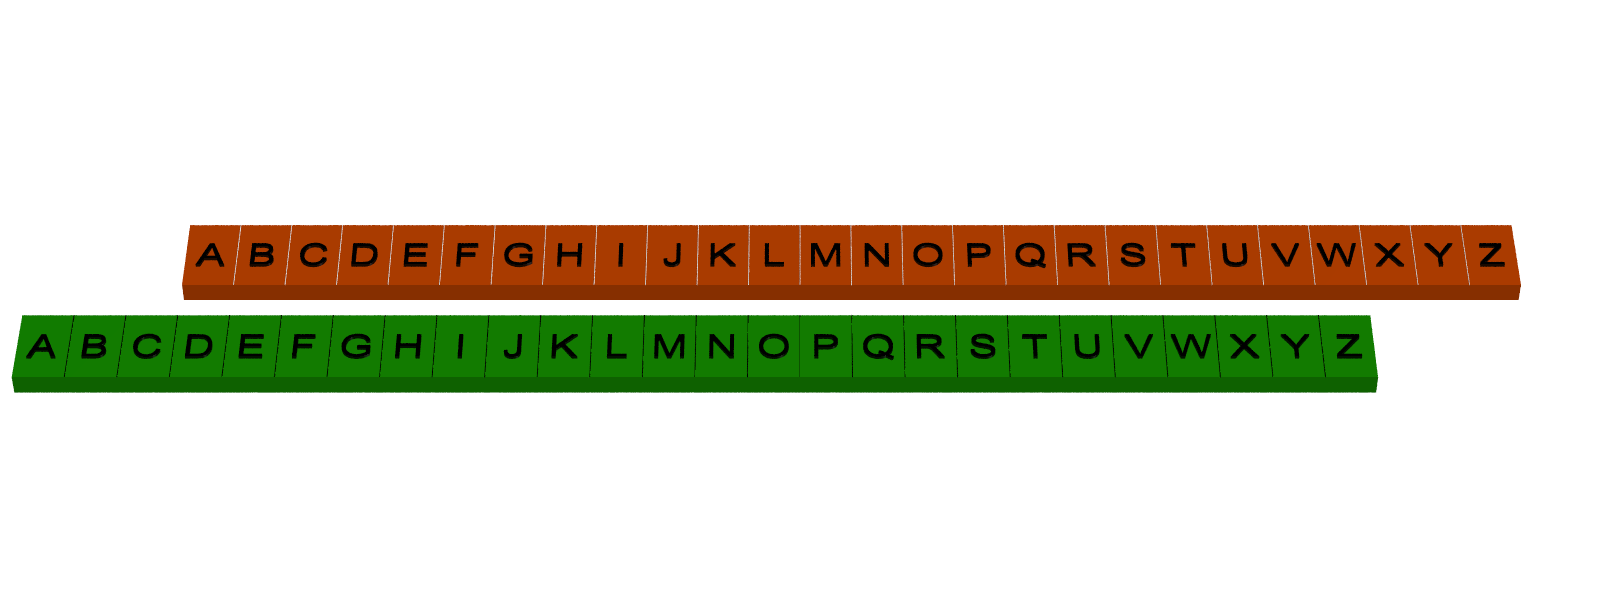
\includegraphics[width=0.9\textwidth]{figures/Cesar_plan_3.png}}


\end{frame}


\begin{frame}

\centerline{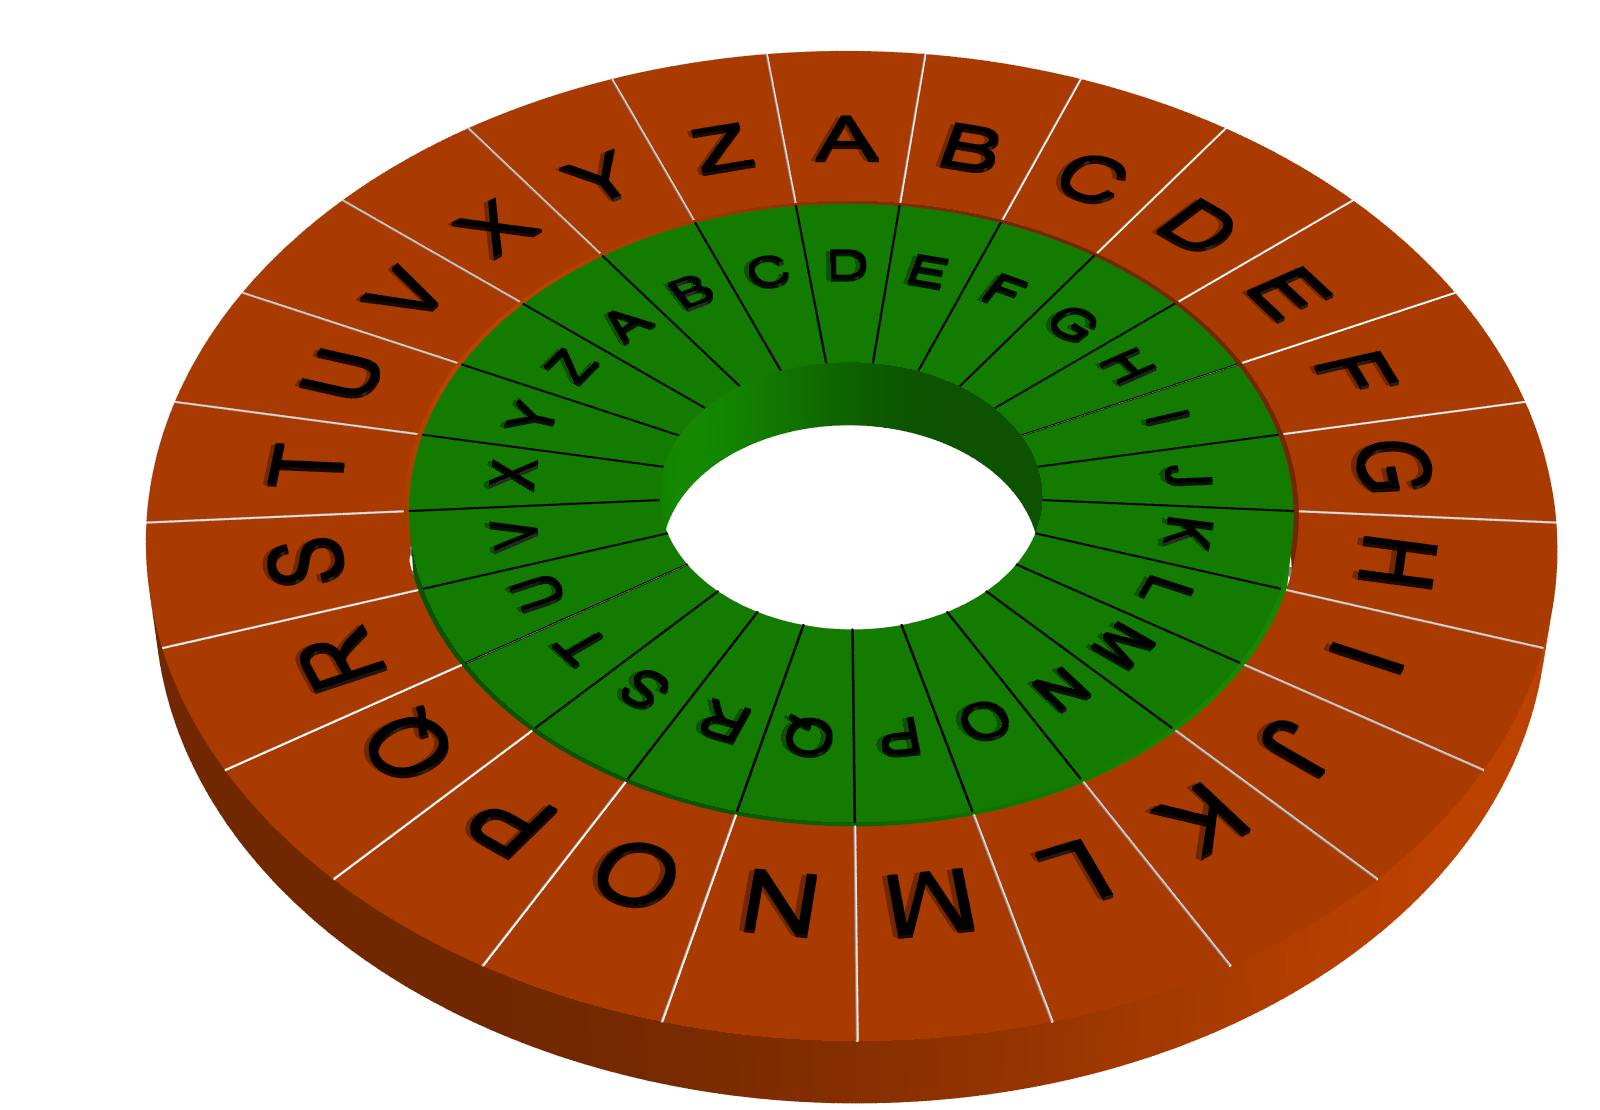
\includegraphics[width=0.5\textwidth]{figures/Cesar_3.png}}

\pause

\begin{itemize}
  \item \defi{Décalage circulaire} sur les lettres de l'alphabet
\pause  
  \item Pour déchiffrer le message de César, on décale dans l'autre sens
\pause  
  \item \public{D} se déchiffre en \prive{A}, \ \public{E} en \prive{B},...
\pause
  \item La phrase de César \\
  \centerline{\public{DOHD \  MDFWD \ HVW}}
  \pause
  devient \\
\centerline{\prive{ALEA \  JACTA \  EST}}
\end{itemize}

\end{frame}




%%%%%%%%%%%%%%%%%%%%%%%%%%%%%%%%%%%%%%%%%%%%%%%%%%%%%%%%%%%%%%%%
\section{Des chiffres et des lettres}

\begin{frame}
\begin{itemize}[<+->]\setlength{\itemsep}{8pt}
  \item On associe aux lettres de $A$ à $Z$ un nombre de $0$ à $25$
  
  \item 
    $$f : \left\{
    \begin{array}{rcl}
    \big\{ A, B, C, \ldots, Z\big\} & \longrightarrow &\big\{ 0, 1, 2, \ldots, 25\big\} \\
    A & \longmapsto & 0\\
    B & \longmapsto & 1\\
    &\vdots&\\
    Z &\longmapsto & 25
    \end{array}
    \right.$$  
  
  \item Exemple : \prive{A L E A} devient \prive{0 11 4 0}
  
  \item Le chiffrement de César est un \defi{chiffrement mono-alphabétique}
  
  \item Il correspond à une opération mathématique très simple
\end{itemize}
\end{frame}




%%%%%%%%%%%%%%%%%%%%%%%%%%%%%%%%%%%%%%%%%%%%%%%%%%%%%%%%%%%%%%%%
\section{Modulo}

\begin{frame}
Fixons un entier $n \ge 2$
\begin{mydefinition}
 On dit que \defi{$a$ est congru à $b$ modulo $n$},
si $n$ divise $b-a$

\pause

On note alors 
\vspace*{-3ex}
$$a \equiv b \pmod n $$ %\pause \qquad \text{ ou } \qquad a \equiv b \pod n
\vspace*{-4ex}
\end{mydefinition}

\pause

\begin{itemize}
  \item $28 \equiv  2 \pmod {26}$\pause, car $28-2$ est bien divisible par $26$
\pause  
  \item $85 = 26+ 59$ donc $85 \equiv  59 \pmod {26}$
\pause  
  \item $85 = 3 \times 26+ 7$ donc $85 \equiv  7 \pmod {26}$
\pause
  \item On note $\Zz/26 \Zz$ l'ensemble de tous les éléments de $\Zz$ modulo $26$
\pause  
  \item Représenté par les $26$ éléments $\{0,1,2,\ldots, 25\}$
\pause
        \begin{itemize}         
          \item $0,\ 1,\ 2,\ \ldots,\  25,$
                \pause 
                \item   puis  $26 \equiv 0,\  27 \equiv 1,  \ldots, \pause 52\equiv0,\  53\equiv1, \ldots$
          \pause    
            \item $-1\equiv25$, $-2\equiv24$,...
            \end{itemize}
\end{itemize}

\pause
\medskip
\begin{itemize}
  \item $\Zz / n \Zz$ contient $n$ éléments
\pause  
  \item Pour $a \in \Zz$, son \defi{représentant} dans $\{0,1,2,\ldots, n-1\}$ est le reste $k$
de la division euclidienne de $a$ par $n$ : $a = bn + k$
\pause
  \item De sorte que $a \equiv  k \pmod n$ et $0 \le k < n$ 
\end{itemize}

\end{frame}


\begin{frame}

\evidence{Addition}
\pause
\begin{itemize}
  \item Pour $a,b \in \Zz/n\Zz$ on associe $a+b \in \Zz/n\Zz$
\pause  
  \item Dans $\Zz/26\Zz$, $15+13$ égale $2$\pause. En effet $15+13 = 28 \equiv 2 \pmod{26}$
\pause  
  \item Que vaut $133+64$ ? 
\pause 
  \begin{itemize}
    \item $133+64 = 197=7\times 26 +15 \equiv 15 \pmod {26}$
\pause    
    \item 
    \begin{itemize}
    \item $133 = 5 \times 26 + 3 \equiv 3 \pmod {26}$
    \pause    
    \item $64 = 2 \times 26 + 12 \equiv 12 \pmod{26}$
    \pause    
    \item $133 + 64 \equiv 3 + 12 \equiv 15 \pmod{26}$
    \end{itemize}
  \end{itemize}

\end{itemize}

\bigskip
\pause

\evidence{Multiplication}

\begin{itemize}
  \item Pour $a,b \in \Zz/n\Zz$ on associe $a \times b \in \Zz/n\Zz$
\pause 
  \item $3\times 12 = 36 = 1 \times 26 + 10 \equiv 10 \pmod{26}$
\pause  
  \item Que vaut $3\times 27$ ? 
  \begin{itemize}
  \item $3 \times 27 = 81 = 3 \times 26 + 3 \equiv 3 \pmod{26}$
  \pause  
  \item $27 \equiv 1 \pmod{26}$ puis $3 \times 27 \equiv 3 \times 1 \equiv 3 \pmod{26}$ 
  \end{itemize}
\end{itemize}


\end{frame}



%%%%%%%%%%%%%%%%%%%%%%%%%%%%%%%%%%%%%%%%%%%%%%%%%%%%%%%%%%%%%%%%
\section{Chiffrer et déchiffrer}

\begin{frame}
\begin{itemize}
 \item La \defi{fonction de chiffrement de César de décalage $k$} ($k$ entier fixé)
\vspace*{-2ex}
\mybox{$C_k : \left\{\begin{array}{rcl}
    \Zz/26 \Zz  & \longrightarrow & \Zz/26 \Zz \\
                x     & \longmapsto & x{\color{red}+k} \\
  \end{array}\right.$}

\pause
Exemple, pour $k=3$ : $C_3(0)=3$, $C_3(1)=4$\ldots


\pause
\medskip

 \item La \defi{fonction de déchiffrement de César de décalage $k$} est
\mybox{$D_k : \left\{\begin{array}{rcl}
    \Zz/26 \Zz  & \longrightarrow & \Zz/26 \Zz \\
                x     & \longmapsto &  x{\color{red}-k} \\
  \end{array}\right.$}
\pause
Exemple : si $1$ a été chiffré en $4$ alors $D_3(4)=4-3=1$

\end{itemize}
\end{frame}
\begin{frame}
\begin{itemize}

 \item $D_k$ est la \evidence{bijection réciproque} de $C_k$

\medskip 
\pause

Pour tout $x \in \Zz/26 \Zz$ \quad
\myboxinline{$D_k \big( C_k(x) \big) = x$}
\end{itemize}

\pause

\begin{center}
\begin{tikzpicture}
  \coordinate (A) at (-1,0);  
  \coordinate (B) at (1,0); 
  \node[left] at (A) {$\Zz/26\Zz$};
  \node[right] at (B) {$\Zz/26\Zz$};
  \draw[->, blue, very thick] ($(A)+(0,0.25)$) to[bend left, thick]node[above, midway]{$C_k$} ($(B)+(0,0.25)$);
  \draw[->, blue, very thick] ($(B)+(0,-0.25)$) to[bend left, thick]node[below, midway]{$D_k$} ($(A)+(0,-0.25)$);  
\end{tikzpicture}  
\end{center}
\end{frame}


\begin{frame}
\hfill\hfill\evidence{Principe du chiffrement}
\pause
\begin{itemize}
  \item Alice veut envoyer des messages secrets à Bruno
  \pause
  \item Ils se mettent sur une clé secrète $k$, par exemple $k=11$
  \pause
  \item Alice veut envoyer le message \prive{COUCOU} à Bruno
  \pause
  \item Elle transforme \prive{COUCOU} en \prive{2 14 20 2 14 20}
  \pause
  \item Elle applique le chiffrement $C_{11}(x)=x+11$ : \public{13 25 5 13 25 5}
  \pause
  \item Mot crypté \public{NZFNZF} transmis à Bruno
  \pause
  \item Il applique la fonction de déchiffrement $D_{11}(x)=x-11$
\end{itemize}

\pause 

\begin{center}
{\scriptsize
\begin{tikzpicture}[scale=0.65]

  \node at (-5,1) {\bf ALICE};
  \node at (5,1) {\bf BRUNO};
  \node at (-7,0) {\prive{COUCOU}};
  \node at (-7,-2) {\prive{2 14 20 2 14 20}};
  \node at (-3,-2) {\public{13 25 5 13 25 5}}; 
  \node at (-3,0) {\public{NZFNZF}};  
  \node at (7,0) {\prive{COUCOU}};
  \node at (7,-2) {\prive{2 14 20 2 14 20}};
  \node at (3,-2) {\public{13 25 5 13 25 5}}; 
  \node at (3,0) {\public{NZFNZF}};
  
  \draw[->, blue, very thick] (-7,-0.25) to (-7,-1.75);
  \draw[<-, blue, very thick] (-3,-0.25) to (-3,-1.75);
  \draw[<-, blue, very thick] (7,-0.25) to (7,-1.75);
  \draw[->, blue, very thick] (3,-0.25) to (3,-1.75);  
  
  \draw[->, blue, very thick] (-6,-1.5) to[bend left, thick]node[above, midway]{$C_k$} (-4,-1.5);
  \draw[<-, blue, very thick] (6,-1.5) to[bend right, thick]node[above, midway]{$D_k$} (4,-1.5);

  \draw[line width=4pt,>=stealth,->,gray] (-1.5,0) to (1.5,0);
\end{tikzpicture}  
}
\end{center}


% \bigskip
% 
% \pause
% 
% \begin{exemple}[Le rot13]
% $$C_{13}(x) = x +13 \qquad \pause D_{13}(x)=x+13$$
% 
% \pause
% \vspace*{-3ex}
% La fonction de déchiffrement est la même que la fonction de chiffrement !
% \pause Exercice : déchiffrez \public{PRFNE} % ["CESAR"]
% 
% \end{exemple}


\end{frame}


%%%%%%%%%%%%%%%%%%%%%%%%%%%%%%%%%%%%%%%%%%%%%%%%%%%%%%%%%%%%%%%%
\section{Espace des clés et attaque}

\begin{frame}
Combien existe-t-il de chiffrements possibles par la méthode de César ?

\pause

\begin{itemize}[<+->]
  \item Il y a $26$ fonctions $C_k$ différentes, $k=0,1,\ldots,25$
  \item $k$ appartient à $\Zz / 26 \Zz$
  \item Exemple : les fonctions $C_{29}$ et $C_3$ sont identiques
  \item Le décalage $k$ s'appelle la \defi{clé de chiffrement}
  \item L'\defi{espace des clés} est
$\Zz/26\Zz$
  \item Sécurité faible
\end{itemize}

\end{frame}


%%%%%%%%%%%%%%%%%%%%%%%%%%%%%%%%%%%%%%%%%%%%%%%%%%%%%%%%%%%%%%%%
\section{Algorithmes}

\begin{frame}[fragile]

\begin{algo}[cesar.py (1)]
\begin{lstlisting}
def cesar_chiffre_nb(x,k):   
    return (x+k)%26
\end{lstlisting}  
\end{algo}

\pause
\bigskip

\begin{algo}[cesar.py (2)]
\begin{lstlisting}
def cesar_dechiffre_nb(x,k):   
    return (x-k)%26
\end{lstlisting}  
\end{algo}

\end{frame}

\begin{frame}[fragile]

{\footnotesize
\begin{algo}[cesar.py (3)]
\begin{lstlisting}
def cesar_chiffre_mot(mot,k):
    mot_crypte = []                                      # Liste vide
    for lettre in mot:                           # Pour chaque lettre 
        nb = ord(lettre)-65             # Lettre devient nb de 0 à 25
        nb_crypte = cesar_chiffre_nb(nb,k)     # Chiffrement de César 
        lettre_crypte = chr(nb_crypte+65)        # Retour aux lettres
        mot_crypte.append(lettre_crypte)   # Ajoute lettre au message
    mot_crypte = "".join(mot_crypte)    # Revient à chaine caractères
    return(mot_crypte)
\end{lstlisting}  
\end{algo}
}

\end{frame}
% 
% \begin{frame}
% 
% Pour chiffrer un mot ou un phrase, il n'y a pas de problèmes théoriques, mais seulement 
% des difficultés techniques :
% \begin{itemize}
%   \item Un mot ou une phrase est une chaîne de caractères, qui en fait se comporte comme une liste.
%   Si \codeinline{mot} est une chaîne alors \codeinline{mot[0]} est la première lettre,
%   \codeinline{mot[1]} la deuxième lettre... et
%   la boucle \codeinline{for lettre in mot:} permet de parcourir chacune des lettres.
%   
%   \item Pour transformer une lettre en un nombre, on utilise le code Ascii qui à chaque caractère 
%   associe un nombre, \codeinline{ord(A)} vaut $65$, \codeinline{ord(B)} vaut $66$... 
%   Ainsi \codeinline{(ord(lettre) - 65)} renvoie le rang de la lettre entre $0$ et $25$ comme nous l'avons fixé dès le départ.
%   
%   \item La transformation inverse se fait par la fonction \codeinline{char} : \codeinline{char(65)} renvoie 
%   le caractère \codeinline{A}, \codeinline{char(66)} renvoie \codeinline{B}...
%   
%   \item Pour ajouter une lettre à une liste, faites 
%   \codeinline{maliste.append(lettre)}. Enfin pour transformer une liste de caractères 
%   en une chaîne, faites \codeinline{"".join(maliste)}.
% \end{itemize}
% 
% \end{frame}




\end{document}
